\documentclass[11pt,a4paper]{article}

% Page layout
\usepackage[margin=2cm]{geometry}
\setlength{\parskip}{0.8em}
\setlength{\parindent}{0pt}

% Fonts and encoding
\usepackage[T1]{fontenc}
\usepackage[utf8]{inputenc}
\usepackage{lmodern}

% Math
\usepackage{amsmath, amssymb, amsfonts}

% Graphics
\usepackage{graphicx}
\usepackage{float}

% Colors and hyperlinks
\usepackage{xcolor}
\usepackage[hidelinks]{hyperref}

% Header and footer
\usepackage{fancyhdr}
\pagestyle{fancy}
\fancyhead[L]{}
\fancyhead[C]{}
\fancyhead[R]{}
\fancyfoot[C]{\thepage}

% Section formatting
\usepackage{titlesec}
\titleformat{\section}{\large\bfseries}{\thesection}{1em}{}
\titleformat{\subsection}{\normalsize\bfseries}{\thesubsection}{1em}{}

% Compact lists
\usepackage{enumitem}
\setlist{nosep}

\usepackage{natbib}

% For two-column layout if needed
% \usepackage{multicol}
% \setlength{\columnsep}{1cm}

% Title info
\title{Determine pinhole size}
\author{J.~M.~O. Massey}
\date{\today}
\begin{document}
\maketitle
\section{Introduction}

    \begin{figure}
        \centering
        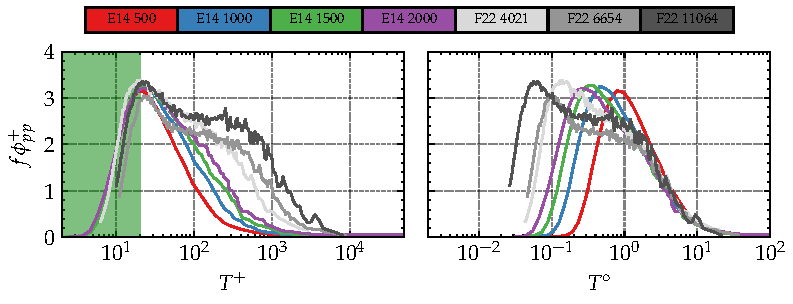
\includegraphics{figures/1_bl.pdf}
        \caption{Inner-scaled, pre-multiplied wall-pressure spectra in inner-(\textbf{left}) and outer-scaled (\textbf{right}) coordinates for a range of Reynolds numbers. The region $T^+\leq 20$ is highlighted in green. Data from \citet{eitel-amor_simulation_2014,fritsch_pressure_2020,fritsch_fluctuating_2022}}
    \label{fig:bl_spectra}
    \end{figure}

    In the measurement of wall pressure fluctuations in a turbulent boundary layer, we use a microphone cap with a pinhole (PH) to avoid spatial attenuation and aliasing effects. To reconstruct the measured pressure, we must callibrate the treated microphone setup and determine a transfer function ($H$) that maps $\mathrm{PH}\mapsto \mathrm{NKD}$, where NKD is the known pressure measurement. If the PH is too small, the suppression of the signal is too much and $H$ is ill-posed.

    Past data has shown that an inner- and outer-scaled part of the premultiplied wall-pressure spectra exist, with the inner-scaled part being invariant to frictional Reynold's number ($\delta^+\equiv \delta u_\tau / \nu$) \citep{massey_eddy_2025}. Figure \ref{fig:bl_spectra} shows that the peak of the inner-function sits at
    %
    \begin{equation}
        T^+\approx 20 ,
    \label{eq: temporal filter}
    \end{equation}
    %
    where the $\bullet^+$ superscript denotes normalisation by viscous length $\nu/U_\tau$. With this region of known behaviour, we can determine the size of the pinhole and correct accordingly.

\section{Spatial approximation using Taylor's frozen turbulence hypothesis}

    Convection velocity can be used to convert temporal fluctuations into spatial structures such that
    %
    \begin{equation}
        c_x^+ \equiv \frac{\omega^+}{k_x^+} \quad \overset{\substack{\omega^+=2\pi f^+\\ k_x^+=2\pi/\lambda_x^+}}{\Longleftrightarrow} \quad \frac{c_x^+}{\lambda_x^+}=f^+ .
    \end{equation}
    %
    Propagating the equality--acknowledging the relationship $T^+\equiv1/f^+$--established in \eqref{eq: temporal filter} leads to
    %
    \begin{equation}
        \frac{\lambda_x^+}{c_x^+}<20
    \end{equation}
    %
    In this context, $\lambda_x^+ \equiv \frac{\ell u_\tau}{\nu}$ is the wavelength of the attenuated structures and $c_x^+$ is the convection velocity of the structures. The convection velocity of the pressure fluctuations is not constant throughout the boundary-layer \citep{willmarth_measurements_1962,corcos_structure_1964}, but a widely adopted approximation is $c_x^+\approx 10$ leading to
    %
    \begin{equation}
        \boxed{\frac{\ell u_\tau}{\nu} < 200.}
    \end{equation}

\section{Viscous scales in the Stanford wind tunnel}

    The plan is to deploy three pinholes, the largest is geared to the atmospheric conditions, the smallest to the highest $\delta^+$, maximum pressure, and one in between. For this study, the boundary-layer thickness is fixed at $\delta = 0.035~\mathrm{m}$ and the free-stream velocity is fixed at $U_{\mathrm{CL}} = 14~\mathrm{ms}^{-1}$.
    
    \begin{table}[H]
        \centering
        \begin{tabular}{c c c}
            $\delta^+$ & $\nu/u_\tau$ [$\mu$m] & $\ell_{\max}$ [mm] \\
            \hline
            1500 & 29.00 & 5.80 \\
            4300 & 7.97 & 1.59 \\
            8200 & 4.00 & 0.80 \\
        \end{tabular}
    \label{tab:stanford}
    \end{table}




\bibliography{refs}
\bibliographystyle{jfm}

\end{document}